\documentclass[12pt]{report}
\usepackage{xcolor} % for different colour comments
\usepackage{parskip} % Space between each paragraph.
%\usepackage{hardwrap} % for text length of 80 pts
\usepackage[margin=1.2in]{geometry}
\usepackage{hyperref}
\usepackage{../ltx/edcomms}
\usepackage{graphicx}
\usepackage[section]{placeins} % Prevents floats from floating across sections
\usepackage{natbib}%Bibtex
\usepackage{float}
\usepackage{tabularx}
\usepackage{ltablex} %% Multi page tables 
\usepackage{booktabs}
\usepackage{tabto}
\usepackage{tocloft} %% This package prevents table of contents from generating a page break
\usepackage{caption}
\usepackage{ifthen}
\usepackage{../ltx/edcomms}

%% Comments are enabled and disabled by 'draft' mode. I hacked in my own draft
%% mode (https://en.wikibooks.org/wiki/LaTeX/Macros) because the LaTeX draft
%% mode disables a bunch of things that I don't want it to. I just want it to
%% disable comments. Do not set any of this manually, just use the build script,
%% which builds both draft and final copies. Comments are enabled by default, so
%% if you build manually, you get a draft copy. 
\providecommand\draftmode{true}

\ifthenelse{\equal{\draftmode}{true}}{
\newcommand{\authornote}[3]{\textcolor{#1}{[#3 ---#2]}}
\newcommand{\todo}[1]{\textcolor{red}{[TODO: #1]}}
%\edcommstrue %% Dr. Kahl's comment package. Eventually we should migrate all
             %% comments to this.
}{
\edcommsfalse 
\newcommand{\authornote}[3]{}
\newcommand{\todo}[1]{}
}

% wss = Dr. Smith ; ds = Dr. Szymczak
\newcommand{\wss}[1]{\authornote{magenta}{SS}{#1}}
\newcommand{\ds}[1]{\authornote{blue}{DS}{#1}}


\usepackage{geometry}
\usepackage{changepage}
\setlength{\parindent}{15pt} % parskip sets this to 0. 15 is default.

\newcolumntype{C}[1]{>{\centering}p{#1}} %% For use with tabularx
%%%%%%%%%%%%%%%	START OF DOCUMENT %%%%%%%%%%%%%%%%%%%%
\edcommsfalse
\begin{document}

\pagenumbering{roman} %% Roman numerals before actual document starts
\begin{titlepage}\begin{center}
\thispagestyle{empty} %% No page no. on title

\vspace*{1cm}

{\Huge\textbf{Ampersand Event-Condition-Action Rules}}

\vspace{0.5cm}
{\Large Software Requirement Specification 
	
	\edinsert{JG}{Version 0}

\vspace{1.5cm}
Yuriy Toporovskyy,\ Yash Sapra,\ Jaeden Guo}
\vfill

We acknowledge that this document uses material from the Volere Requirements
Specification Template, copyright 1995 - 2012 the Atlantic Systems Guild
Limited.

\vspace{0.8cm}
\end{center}
CS 4ZP6 \\
October 9th, 2015 \\ 
Fall 2015 / Winter 2016 
\end{titlepage}

%% Revision history

\begin{table}[ht!]\begin{center}
\caption{Revision History}  
\begin{tabular}{|l|l|l|}\hline
\textbf{Author} & \textbf{Date} & \textbf{Comment} \\\hline 
Yuriy Toporovskyy & 26 / 09 / 2015 & Initial skeleton version \\\hline
Yuriy Toporovskyy & 30 / 09 / 2015 & Project drivers, description and \\ & & 
added project diagram and project flow chart \\\hline
J Guo & 09 / 10 / 2015 & Update: Non-Functional first half 4.1-4.3, added to 
1.2.2, \\ & & completed 2.2 \\\hline
J Guo & 13 / 10 / 2015 & Update: Figures added for Non-Functional 4.1-4.7,  \\ 
& & 
Non-Functional second half 4.4-4.7 half, \\ & & added Functional 3.3 - System 
requirements  and \\ 
& & diagram figure, \& Section 5.8 \\\hline
Yash Sapra &  12/ 09 / 2015 & Non-Functional - legal requirements, \\ & & Functional - User 
Requirements, tasks, risks \\ & & and chapter 5.
\\\hline
Yuriy Toporovskyy & 13 / 10 / 2015 & Initial round of editing \\\hline
\end{tabular}
\end{center}\end{table}

\newpage

\tableofcontents
\listoffigures
\listoftables

\newpage
\pagenumbering{arabic} %% Arabic numerals in actual document

%%%%%%%%%%%%%%%%%%%%%%%%%%%%%%%%%%%%
%% Chapter 1: ???                 %%
%%%%%%%%%%%%%%%%%%%%%%%%%%%%%%%%%%%%
\setlength{\arrayrulewidth}{0.35mm}
\setlength{\tabcolsep}{16pt}
\renewcommand{\arraystretch}{2}
\begin{figure}
	\begin{adjustwidth}{-1cm}{}
	\begin{tabular}{ |m{4cm}|m{6cm}|m{4cm}|  }
		\hline
		\multicolumn{3}{|c|}{\bfseries{Project Time Table}} \\
		\hline
		\bfseries{Projected Finish Date}& \bfseries{Milestone} & 
		\bfseries{Actual Finish Date} \\
		\hline
		 09/10/2015& EFA SRS version 0 & 13/10/2015 \\
		19/10/2015 & EFA SRS version 1  & 22/10/2015 \\
		23/10/2015 & Proof of Concept Demonstation & 19/01/2016 \\
		10/02/2016 & Software Demonstration & 10/02/2016 \\
		--- & --- & --- \\
		01/04/2016 & EFA Complete & --- \\
		\hline
	\end{tabular}
	\end{adjustwidth}
\end{figure}
\chapter{Ampersand As A System}\label{ch:Intro}


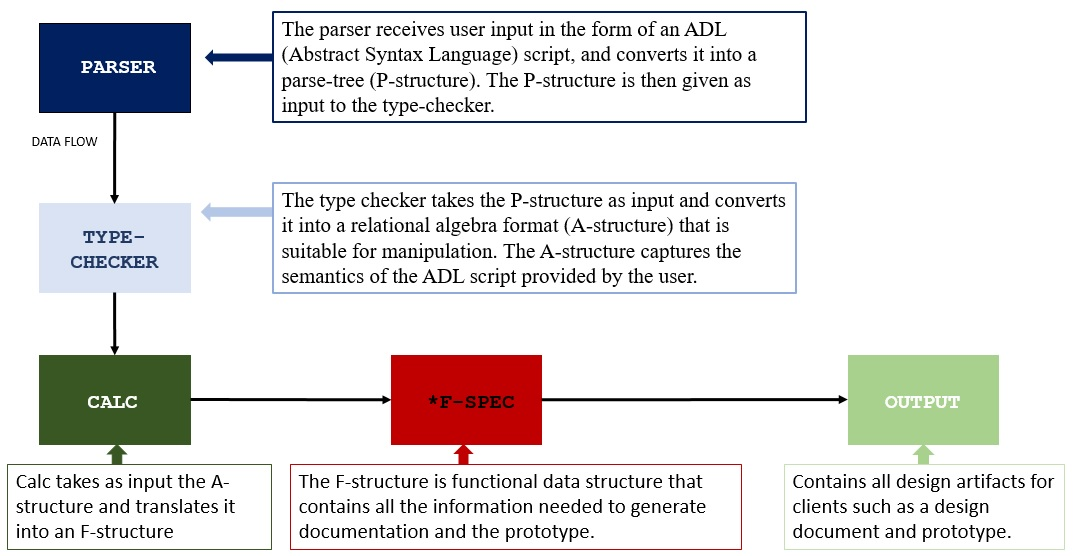
\includegraphics[width=\textwidth]{../figures/ampersand_parts}
\paragraph{}
Ampersand is an open-source project that produces design artifacts based on 
business rules. One of the essential functions of Ampersand is to maintain all 
the business rules that keep transactions valid during the course of each 
cycle, where multiple transactions could take place.  The diagram above breaks 
down the major components of ampersand ignoring specification details. This 
project focuses mainly on one component of Ampersand, which is the F-spec which 
contains ECA/(Event-Condition-Action Rules/) that each process must obey. These 
rules are essential to the functionality of ampersand, and purpose of this 
project is to correctly translate ECA Rules into type safe SQL queries.
{\section{The Ampersand Environment}\label{sec:Purpose}}
Ampersand is a on-going project with an increasing number of modules being
added to it on a weekly basis. Since this project focuses on a component of 
ampersand, it must be built to fit within the ampersand environment and 
co-exist with other modules. Due to this restriction, many design decisions are 
predetermined such as types of data that are used and programming language used 
to build them.
\subsection{Project Purpose}
The purpose of this project is to correctly translate ECA rules, used to 
maintain business conditions into type-safe SQL queries using Haskell. 
\subsection{Project Goals} 
The goals of this project can be divided into two components. The first 
component consists of satisfying the condition necessary for the completion of 
an undergraduate capstone project. The second component is to design and 
implement maintainable code that can be absorbed to the ampersand open-source 
project. 
\section{The Stakeholders}\label{sec:Stakeholders}
The stakeholders is separated into two sections, those that directly benefit 
from this projects contribution and those that indirectly benefit.
\subsection{Ampersand Designers}\label{subsec:Ampersand}
Ampersand designers is our client, and they directly benefit from this project 
as it bring Ampersand one step closer to completion. This project EFA /(ECA for 
Ampersand/) delivers a maintainable component for Ampersand that produces type 
safe SQL queries, a crucial part of Ampersand used for database manipulation 
which is currently absent. 

\subsection{End-Users}\label{subsec:BusReq}
\paragraph{}
Ampersand users indirectly benefit from this project's contribution because it 
drastically decrease the time spent manually restoring system invariants, which 
are the rules that maintain the validity of each business process. As EFA is 
executed during compile time, the user will not suffer any noticeable delays 
and can rest assured that the artifacts they received are correct according to 
specification.

%%%%%%%%%%%%%%%%%%%%%%%%%%%%%%%%%%%%
%% Chapter 2: Project Constraints %%
%%%%%%%%%%%%%%%%%%%%%%%%%%%%%%%%%%%%
\chapter{Project Constraints}\label{ch:Constraints}
The current Ampersand system is the main limitation of this project; everything 
that is built, must be built to fit within its current constraints. These 
constraints include the language used to build Ampersand /(i.e. Haskell/). 
Anything incorporated into Ampersand must be implemented in the Haskell 
language as other languages cannot be used. Additional constraints is placed on 
the acceptance of this project by our clients, which is to produce maintainable 
code; this includes the use of dependable libraries and any support modules 
generated by this project to help the translation of ECA rules to SQL commands.

\section{Mandated Constraints}\label{sec:Constraints}
%%%%
%% 4.1 Solution constraints. 

All code must be well documented, backwards compatible and fit seamlessly into 
the current Ampersand project. Due to the long-term nature of this project, we 
must minimize the number of external dependencies as we little, if any control 
over the modification that will be made to them over time. 

%%3b.
\subsection{Implementation Environment of the Current System}
\subsubsection*{Haskell}
The Ampersand code base is written almost entirely in Haskell 
(\cite{ampSource}) with the exception of user interfaces for the generated 
prototypes written in PHP and Javascript. Haskell is the only programming 
language we can use to build modules for ampersand.


\subsubsection*{The Glasgow Haskell Compiler \& Cabal Build System}
As most of Ampersand's base code is written in Haskell, a compiler must be used 
to compile it. The Glasgow Haskell Compiler (\cite{GHC}) with the Cabal build 
system (see \verb|ampersand.cabal| must be used to compile ampersand 
\cite{ampSource}). Ampersand is not designed to used with other Haskell 
compilers.


\subsubsection*{GitHub Repository}
Ampersand's main repository is hosted on github, we must also host our project 
on github to be able to maintain consistency with the Ampersand source code.

\subsubsection*{Graphviz}
Graphviz is an open source graph visualization software, which can
visually represent information in the form of charts and graphs. Graphviz is 
used to create visuals in ampersand artifacts and is an essential to running 
ampersand.

\subsubsection*{XAMPP}
XAMPP is used to create a local ampersand database for the generated prototype. 
Ampersand is internally built to use XAMPP configurations, and currently it is 
not set up to use alternative software for database generation.

\subsection{Partner of Collaborative Applications}
%%3c. of voltere template, applications that are not part of product but with 
%%which the product will collaborate, can be external applications, commercial 
%%packages or pre-existing in-house applications
\begin{longtable}{ |m{4.5cm}|m{1.5cm}|m{7cm}|  }
    \hline 
    \textbf{Name} & \textbf{Type} & \textbf{Description} \\ \hline \hline
    AbstractSyntaxTree & Ampersand module & A module designed specifically for 
    Ampersand, data from this module is manipulated in EFA.
    \\ \hline        
    Control.Applicative & Library module & An interface that provides an 
    intermediate structure between a monad and a functor. This interface is 
    used to embed pure expressions, sequence computations and combine their 
    results.  \\ \hline
    Control.Exception & Library module & An interface that provides support for 
    raising and catching build-in and user-defined exceptions.  \\ \hline
    Control.DeepSeq & Library module & This module is used to fully evaluate 
    data structure and is used to prevent resource leaks in lazy IO programs.  
    \\ \hline            
    Data.Proxy & Library module & A concrete proxy type, used to represent the 
    value of something else.  \\ \hline    
    Data.Type.Equality & Library module & This module offers pattern-matching 
    on types and provides a proof, it is used as a definition of propositional 
    equality.  \\ \hline        
    Data.List & Library module & A module that provides support for operations 
    on list structures.  \\ \hline
    Data.Char & Library module & A module that provides support for characters 
    and operations on characters.  \\ \hline
    Data.Coerce & Library module & Provides safe coercions between data types; 
    allows user to safely convert between values of type that have the same 
    representation with no run-time overhead.   \\ \hline
    Debug.Trace & Library module & Interface for tracing and monitoring 
    execution, used for investigating bugs and other performance issues.  \\ 
    \hline
    GHC.TypeLits & Library module & Internal GHC module that declares the 
    constants used in type-level implementation of natural numbers.  \\ 
    \hline    
    GHC.Exts & Library module & This modules allows the use of pointers to an 
    object or array of objects.  \\ \hline    
    Language.SQL.SimpleSQL & Library module & Syntax: provides the AST for SQL 
    queries. \\& & Pretty: provides pretty printing functions that formates 
    output for human reading. \\ \hline            
    Numeric.Natural & Library module & Natural number type  \\ \hline    
    Prelude & Library module & A standard module that is imported by default 
    and provides support for basic data types, comparison functions, and 
    methods used for data manipulation.   \\ \hline
    System.IO.Unsafe & Library module & This module allows IO computation to be 
    performed at any time, the IO computation must be free of side effecets and 
    independent of its environment to be considered safe. Any I/O computation 
    that is wrapped in unsafePerformIO performs side effects.  \\ \hline
    Text.PrettyPrint.Leijen & Library module & A pretty printer module based 
    off of Philip Wadler's 1997 "A prettier printer", used to show SQL queries 
    in a readable manner to humans.  \\ \hline        
    Unsafe.Coerce & Library module & A helper module that converts a value from 
    any type to any other type, the user must assure that the old data type and 
    the new data type have identical internal representations, else runtime 
    corruption occurs. This is used in the translation of ECA rules to SQL 
    using unique data types.  \\ 
    \hline  
\end{longtable}
\section{Naming Conventions and Terminology}\label{sec:Naming} 
\begin{description}
\item[ECA] Stands for Event-Condition Action. The rule structure used for data
  bases and commonly used in market ready business rule engines. ECA rules are
  used in Ampersand to describe how a database should be modified in response to
  a system constraint becoming untrue.
  
\item [ADL] Stands for ``Abstract Data Language'' (\cite[13]{derFun}). From a
given set of formally defined business requirements, Ampersand generates a
functional specification consisting of a data model, a service catalog, a
formal specification of the services, and a function point analysis. An ADL
script acts as an input for Ampersand. An ADL file consists of a plain ASCII
text file.
\item [Ampersand] Ampersand is a method and the name of the open source 
project. 
    \begin{itemize}
        \item[$\Rightarrow$] The Ampersand method is used to generate
        functional specification from formalized business requirements.
        \item[$\Rightarrow$] The Ampersand software is a tool that implements 
        this method.
    \end{itemize} 
    
\item [Business rules] Rules that exist to represent real world 
constraints that the virtual world does not naturally possess, such as resource 
and social limitations. Examples of constraints include but are not limited to 
financial, logistic, physical or legal constraints.

\item [EFA] Stands for ``ECA (see above) for Ampersand''. This term is used to 
refer to this project. 
\item [Functional specification] A \emph{formal} document which details the 
operation, capabilities, and appearance of a software system. 

\item [Natural language] Language written in a manner similar to that of human 
communication; 
  language intended to be interpreted and understood by humans, as opposed to 
  machines. 
  
\item [Requirements engineering] The process of translating business
requirements into a functional specification. 
\end{description}

\section{Relevant Facts and Assumptions}\label{sec:Assumptions}
This project makes the assumption that Ampersand users are using it according 
to its intended purposes and have all the necessary software dependencies 
installed for it properly function. This project is designed with the 
assumption that no direct interaction is necessary between the design component 
and the user. All interactions that could take place is buffered by Ampersand. 
Furthermore, we assume that Ampersand users are industry professionals that are 
capable of tracing error messages and fixing them. 

\subsection{Error Detection}
EFA provides traceable error messages for the developer, however on a user 
level these trace error messages would be absorbed into Ampersand and its 
various error detection mechanisms situated on every level of compilation. 
Ampersand is equipped with friendly error detection for the user beginning with 
syntax detection for ADL scripts to assure that there are no missing or out of 
place components. To logical error detections that the user might have missed 
during the creation of their information system. The error messages inform the 
user what line the error has been found, what the error pertains to, and what 
is expected typically in the script structure. The script structure provides 
the user clues for how they may wish to fix the error by adjust their script to 
fit the appropriate format.

%%%%%%%%%%%%%%%%%%%%%%%%%%%%%%%%%%%%%%%%%%
%% Chapter 3 -- Functional requirements %%
%%%%%%%%%%%%%%%%%%%%%%%%%%%%%%%%%%%%%%%%%%
\chapter{Functional Requirements}\label{ch:Functional}
\begin{figure}[!htb]
    \begin{center}
        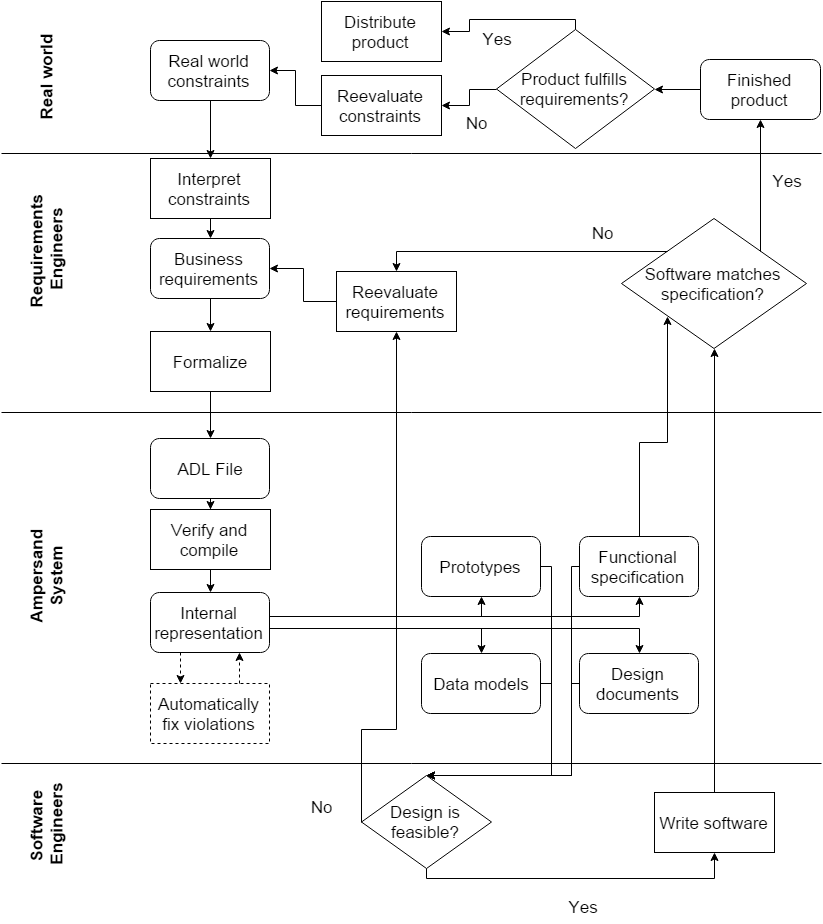
\includegraphics[width=\textwidth]{../figures/business_process}
        \caption{Business process diagram representing the role of Ampersand in 
        the software design cycle}~\label{fig:BusinessProcess} \end{center}
The diagram is a simplified view of the software design cycle, intended to 
highlight 
the role of Ampersand in this cycle. This view omits many of the uses of the 
design artifacts generated by Ampersand; instead it focuses mainly on the 
primary purpose, which is to help create a finished software system. 

The contribution of this project is denoted with dashed lines. Note that it is
isolated to a process completely internal to Ampersand.    
\end{figure}


\section{The Scope of the Work}\label{sec:ScopeOfWork}
\textit{The following sections focuses specifically on EFA and how it will 
function in the Ampersand environment.}
%data flow diagram for EFA goes here
EFA is an automated process internal to Ampersand, and as a part of the 
ampersand system it works in collaboration with other internal components such 
as the F-spec. The purpose of EFA is to replace the current exec-engine, 
creating a permanent solution for the implementation of ECA rules. EFA also 
provides extensive functionalities that the exec-engine is missing, such as the 
ability to manipulate data in a database beyond the basic level of creating and 
dropping tables, and basic select queries. It provides the fundamental 
datatypes that are crucial for the expansion and maintenance of Ampersand as it 
grows. Due to the way that queries are generated in its present state, large 
number of projects will bog down the system until it becomes unmanageable, and 
if Ampersand is used in practice.

\subsection{The Current Situation} %what is being replaced/made better, the 
%effects of the proposed change

Ampersand currently has an exec-engine that passes SQL queries which are 
triggered by the prototype user interface implemented in PHP. Though the 
exec-engine functions, it is a temporary solution for translating ECA rules 
into SQL queries. Any changes made to the information system after its initial 
generation require manual maintenance. This project will create a permanent 
solution that is provably correct and will automate the correction of system 
invariants so that manual maintenance of system invariants is no longer 
necessary once EFA has been successfully incorporated into Ampersand.

\section{The Scope of the Product}\label{sec:ScopeOfProduct}
The translation of ECA rules into SQL queries require unique datatypes that 
preserves the semantics the user provides in the ADL script. ECA rules are 
generated from the conditions the user specifies in the ADL script. The SQL 
queries generated from ECA rules can be thought of as a sequence of changes 
made to the data. This sequence of actions are made through specific event 
triggers, and the actions only take place if all conditions are satisfied and 
are valid. An example of this, would be attempting to delete a person who does 
not exist. This actions cannot be completed because the person does not exist, 
this action would be invalid. 

\section{Functional Requirements}\label{sec:Functional}
\ds{What about error handling on the new contributions?
    Where's the functional requirement related to: 
    ``be a pure function; it should not have side effects." and 
    ``provide diagnostic information about the algorithm to
    the user, if the user asks for such information."?}

\subsection{System Requirements}
%%-----------------------------SIDE EFFECTS---------------------------------%%
{\setlength{\tabcolsep}{12pt} %% Default is 6
    \begin{tabularx}{\textwidth}{>{\bfseries}m{3cm}X}
        Requirement & S1 \\ 
        \midrule
        \endhead
        Description  & Create pure functions with no unintended side effects
        \\	Rationale & The use of a functional programing languages requires 
        that this program be a pure function and does not have side effects, 
        however certain portions of the code requires the execution of side 
        effects to match the behaviour presented by external programs. In these 
        specific instances, the side effects are an intended behaviour.
        \\	Originator & Stakeholder/Developer
        
        \\	Fit Criterion & This behaviour is necessary to produce the results 
        the stakeholders desire
        \\ Test Case & Desired results can be confirmed as they will be 
        reflected in changes that take place in the ampersand database.
        \\	Customer Satisfaction & 5 - Highest 
        \\	Priority & 5 - Highest 
        \\	Supporting Materials & (Rule Based Design \cite {RBD})
        \vspace{12pt}
    \end{tabularx}
}

%%------------------USE OF HASKELL AS IMPLEMENTATION LANGAUGE-----------------%%
{\setlength{\tabcolsep}{12pt} %% Default is 6
    \begin{tabularx}{\textwidth}{>{\bfseries}m{3cm}X}
        Requirement & S2 \\ 
        \midrule
        \endhead
        Description  & The use of Haskell to implement EFA modules
        \\	Rationale & The source code of Ampersand is written completely in 
        Haskell, and thus Haskell must be used for any modules created by this 
        project to be absorbed into the pre-existing source code.
        \\	Originator & Ampersand Creators (i.e. our client)        
        \\	Fit Criterion & Primary ability to write code compatible with 
        Ampersand as it is.
        \\ Test case & Added modules are tested with cabal build inside of 
        Ampersand
        \\	Customer Satisfaction & 5 - Highest 
        \\	Priority & 5 - Highest 
        \\	Supporting Materials & Dr. Joosten, Joosten and Kahl
        \vspace{12pt}
    \end{tabularx}
}
%%------------------ MODULES MUST FIT AMPERSAND FRAMEWORK-----------------%%
{\setlength{\tabcolsep}{12pt} %% Default is 6
    \begin{tabularx}{\textwidth}{>{\bfseries}m{3cm}X}
        Requirement & S3 \\ 
        \midrule
        \endhead
        Description  & Added modules must fit within Ampersand's current 
        framework
        \\	Rationale & As Ampersand is a huge system that has weekly additions 
        to prevent conflict and breaking of existing packages/modules, an 
        effort should be made to minimize external dependencies. As EFA will be 
        an internal component of Ampersand, if a package that EFA depends on to 
        function properly is no longer maintained and breaks, it will in turn 
        break Ampersand.
        \\	Originator & Ampersand Creators (i.e. our client)        
        \\	Fit Criterion & Functionality of EFA as an Ampersand internal 
        component.
        \\ Test case & Added modules are tested with cabal build inside of the
        Ampersand system as an internal component (i.e. System testing)
        \\	Customer Satisfaction & 4 - High 
        \\	Priority & 4 - High
        \\	Supporting Materials & Hackage, Dr. Kahl
        \vspace{12pt}
    \end{tabularx}
}

\subsection{Project Requirements}
%%-------------------------TYPE CORRECTNESS ----------------------------------%%
{\setlength{\tabcolsep}{12pt} %% Default is 6
    \begin{tabularx}{\textwidth}{>{\bfseries}C{3cm}X}
        Requirement & P1 \\ 
        \midrule
        \endhead
        Description  & Provable Correctness: Haskell like other functional 
        programming languages have 
        a strong type system which can be used for machine-checked proofs.
        \\	Rationale & Curry-Howard correspondence which states that the 
        return type of the function is analogous to a logical theorem, that is 
        subject to the hypothesis corresponding to the types of the argument 
        values that are passed to the function and thus the program uysed to 
        compute that function is analogous to a proof of that theorem.
        \\	Fit Criterion & Provable correctness of the program that is 
        generated.
        \\ Test Cases & Internal structure of ECA rules can be compared to SQL 
        queries through a series of datatype tests, each of which will result 
        in a traceable result or error message
        \\	Priority & 4 - High
        \\	Supporting Materials & Programming language theory, Dr. Kahl
        \vspace{12pt}
    \end{tabularx}
}
%%--------------------------CORRECTNESS OF ECA TO SQL RULES ------------------%%
{\setlength{\tabcolsep}{12pt} %% Default is 6
    \begin{tabularx}{\textwidth}{>{\bfseries}C{3cm}X}
        Requirement & P2 \\ 
        \midrule
        \endhead
        Description  & Generated SQL queries must preserve the semantics of ECA 
        rules.  
        \\	Rationale & The translation would otherwise not be correct, as the 
        rules would be meaningless if their semantics are lost.
        \\	Originator & Ampersand Developers
        \\	Fit Criterion & Generated queries must be provably correct as per 
        client's request.
        \\ Test Cases & Internal structure of ECA rules can be compared to SQL 
        queries through a series of datatype tests, each of which will result 
        in a traceable result or error message
        \\	Priority & 4 - High
        \\	Supporting Materials & Hackage, Dr. Kahl
        \vspace{12pt}
    \end{tabularx}
}
%%-------------------------TRACABLE EERRORS---------------------------%%
{\setlength{\tabcolsep}{12pt} %% Default is 6
    \begin{tabularx}{\textwidth}{>{\bfseries}C{3cm}X}
        Requirement & P3 \\ 
        \midrule
        \endhead
        Description  & Generating traceable results and error messages for 
        handling new contributions from this project
        \\	Rationale & Saves time by allowing the program to inform the 
        programmer where the errors are located.
        \\	Originator & Ampersand Developers
        \\	Fit Criterion & Errors must be traceable and have a standard format 
        that can be easily followed.
        \\ Test Cases & Error message will print to screen.
        \\	Priority & 4 - High
        \\	Supporting Materials & Hackage, Dr. Kahl
        \vspace{12pt}
    \end{tabularx}
}

\subsection{Non-Functional Requirements}
%%---------------------------AVAILABILITY TO USERS REQUIREMENT ---------------%%
{\setlength{\tabcolsep}{12pt} %% Default is 6
\begin{tabularx}{\textwidth}{>{\bfseries}C{3cm}X}
Requirement & N1 \\ 
\midrule
\endhead
Description  & EFA must be available at anytime ampersand is running.
\\	Rationale & To provide the user with unlimited access to EFA within 
Ampersand.
\\	Originator & Ampersand Developers
\\	Fit Criterion & Ampersand can detect when internal components are 
non-responsive
\\ Test cases & Ampersand is subject to sentential tests on a daily basis as 
part of its maintenance.   
\\	Priority & 4 - High
\\	Supporting Materials & Useful feedback in Ampersand parser \cite{SB2011}
\vspace{12pt}
\end{tabularx}
}


\chapter{Non-functional Requirements}\label{ch:NonFunc}
\begin{figure}[!htb]
	\centering
	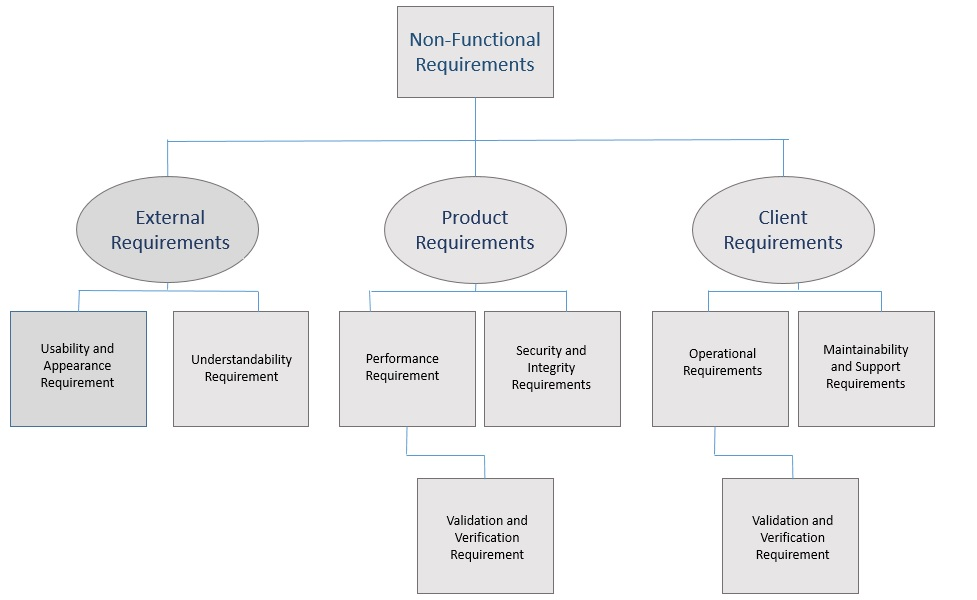
\includegraphics[width=0.8\textwidth]{../figures/NONFUNCTIONAL}
	\caption{Tree of non-functional requirements as it relates to EFA}~\label{fig:figure2}
\end{figure}
\section{Usability and Humanity Requirements}\label{sec:Usability}
\textit{This section is not directly related to EFA, but rather Ampersand.}
\subsection{Administrators}
Administrations are the primary end users that create the ADL script and any 
individual who can use Ampersand can or will be automatically using EFA. 
Administrators in particular have full system access and will use EFA whenever 
the system requires change. No users interact with EFA, but if usability is 
extended to Ampersand, it is a rather complicated system to navigate and is 
geared towards industry professionals. Those ages 21 and under are unlikely to 
use this product. Users seeking to be administrator should have a basic 
understanding of programming.
\subsection{Ordinary Users}
This section covers the majority of individuals who are able to use the 
artifacts that Ampersand produces, such as the prototype interfaces which are 
very use friendly for all those who are 12 years of age and over and computer 
literate.

\section{Understandability}
\paragraph*{}
What EFA does is simple to understand: it fixes logical inconsistencies with 
minimal, if any,input from the user. It does this by looking for 
contradictions, or violations. This product will use natural language that is 
easy to understand when error reporting and hide the details of its 
construction from the user. Any symbols that are not standard mathematical 
symbols will be explained and a full range of mathematical symbols are 
explained in detail in the Ampersand User Guide. 

An example is given as to how a decision making process takes place: there is a 
red chair, there is a blue chair, but there is only one chair. That chair 
cannot be blue and red simultaneously; to fix the problem, either another chair 
is added or one of the colour conditions is eliminated. What is eliminated may 
be based on what is more important for the system and the user. In the previous 
example, if it is most important that there is only one chair, then one of the 
colours statements is erased. 

It may pick a chair colour depending on another criteria that comes from another
part of the information system. For example, if majority of customers' 
favourite colour is red,then most individuals who may use the
chair would prefer it to be red rather than blue. Ampersand is built to keep 
external conditions in mind and those conditions are passed along to EFA. EFA 
can recognize if any of these conditions are violated and may return a message 
to the user concerning what was modified based on what conditions. %% Does 
%%it? Is this an accurate descrition of the system?
%% That may be an external condition
%% that Ampersand has been programmed to keep in mind.
\begin{figure}
	\centering
	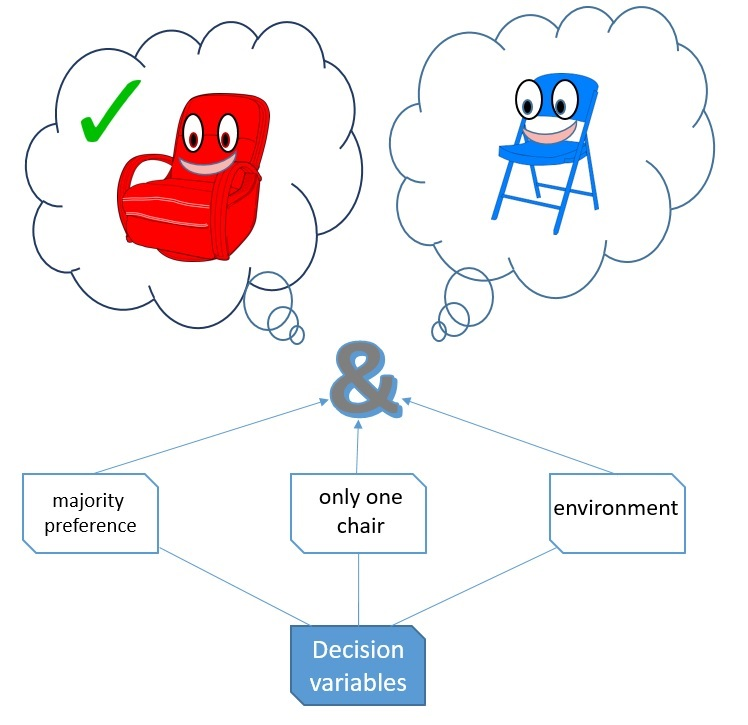
\includegraphics[width=0.5\textwidth]{../figures/blueorredchair}
	\caption{Simplistic diagram of decision making process}
  {\captionsetup{font=small}\caption*{Note: For this process, the blue chair is 
  discarded, we can think of it as the deletion of a dataset that contradicted 
  one or more of the conditions that the user specified. In this case, a 
  message may be returned such as: \\ \textbf{Based on condition} : "can only 
  have one 
  chair", 
  "higher precentage of users prefer the use of red chair". \\ 
  \textbf{modified:} deletion of blue chair, retain red chair. \newline 
  \textit{ Each condition is seperated by a 
  comma, and each action taken to modify the existing system is also seperated 
  by a comma. \\ The original dataset is always preserved thus any changes can 
  be reverted if they are deemed undesirable, however if the user decides that 
  they would like to keep the changes that are made. They are prompted 
  \big(e.g. Would you like to keep current changes? \big) and the most current 
  copy is saved over previous copies. In either circumstance the original input 
  data created by the user is kept as "before" version.)}
  \ref{fig:figure5}}~\label{fig:figure4}}
\end{figure}

\ds{What are your understandability requirements for this project?}

\section{Performance Requirements}\label{sec:Performance}
\paragraph*{}
Ampersand can efficiently process a large amount of information in a short 
amount of time; and the process that EFA requires will be added onto 
Ampersand’s process time. The time it would take to verify data inconsistencies 
would depend on the complexity of the system design and the number of 
corrections it may take to update the system to a valid prototype according to 
specification. Any interface between a user and the automated system shall have 
a maximum response time of 1 minute. The response time shall be faster after 
the initial compilation to avoid breaking the user's flow of thought. The 
system shall prevent deadlock and cycling by flagging areas that it has already 
corrected. 

The prototypes termed "simple models" are tasks that can be accomplished by an 
individual within a short amount of 
time, such as selecting the best actor/actress to play lead according to 
experience and audience appeal. Simple models are able to take into 
consideration not only the task at hand but the context 
and environment to which the task must be completed in. Performance is measured 
on speed, but also on validation of limitations set forth by the user; it will 
not matter how quickly EFA can do something if it does it incorrectly and 
creates more work for the user. Currently, the quantification of the desired 
accuracy of the results produced is unknown, as EFA is in its initial stages. 
Furthermore, the allowable time between failures is unknown and untested.

EFA can be a great tool, but in case of failure, in the unlikely event that 
errors are propagated through the system and no one through any cycle of 
development catch it. If the designer puts full faith in EFA it could be 
catastrophic, especially if mistakes are not caught and products proceed into 
the production stage (\cite[153]{RBD}). However, our contribution will include 
the propogation of proofs as well as feedback to the user. These proofs
will be generated based on the algorithm used by EFA. These proofs will be
human-readable, so that if an engineer suspects that EFA has made a mistake, she
can examine the proof to be convinced that EFA is indeed sound. If the proof
contains a mistake, it will be much easier to catch than a code error. 

\ds{Explicitly state your performance requirements. Also, fix the odd break in
the last paragraph.}

%%Figure removed - unreferenced and unexplained Figure.

%%	YS
%% 	Does this image aboe (^^) belong here? I believe this is the Figure 5.4 that is related to role of Ampersand in the INDiGO proj
%%	 I suggest the following changes, in support of Dr. Joosten's comments
\edcomm{YS}{ECA rules can have interdependencies, these might be buried deep into the rules. Following a certain course of action under EFA, can trigger a deadlock situation where in the system is not able to come up with the best way to deal with inconsistencies in data. In the above example lets say the system is required to give a 2$ discount to the customer if the total cost(including) of his basket is greater than or equal to $10 and provide free shipping, but if the total cost (after discount ) is less than 10$ then 2$ needs to be added for shipping. This creates an infinite loop where the initial cost of the chair is a discount to $8 but then shipping is applied, and it becomes $10, which is again subjected to the discount. EFA needs to take care of such performance issue that would lead the system into a state if deadlock. EFA must have a run time capability to interrupt and send a message to the user about the existence of such conflicting requirements.
}
\edcomm{JG}{feel free to add that}
%%	I'm not too sure if the example is valid in our case, Does Ampersand automatically detect such conflicting requirements at an
%%	early stage? I've belive the existence of relational algebra can detect such conflicts, but what if they are introduced at run
%%	later, while the information system is in production?

%% Can you guys come up with a better example? The ones we've listed before don't really capture the performance of EFA

\section{Operational and Environmental Requirements}\label{sec:Operational}
\paragraph*{}
Any system that is currently running Ampersand will be able to run this product 
under a new verion and thus no new requirements have been introduced.
\ds{Either explicitly state the current requirements for running Ampersand, or
mention that any system currently running Ampersand will be able to run
the new version and thus no new requirements have been introduced}.

\section{Maintainability and Support Requirements}\label{sec:Support}
\paragraph*{}
All code submitted for this project must be maintainable, which mean it is well 
documented and comes with mathematical proof. This is an essential requirement 
for the future maintenance of Ampersand. EFA must make sure that each 
specification/error is traceable (\cite[2]{derFun}).

\edcomm{who}{Part of the reason that non-functional requirements as essential 
to EFA concerns the requirements for interfacing with Adjacent Systems. Thus 
features concerning how implementation is done which is normally based on the 
choice of the designers is a functional requirement when it comes to EFA }
%%YS - 	I don't think the above commented lines are related to EFA or it maintainability.
%%		I don't think they belong here.
  
\ds{Pull out the explicit requirements and remove the fluff.}

\section{Security and Integrity Requirements}\label{sec:Security}
\edcomm{JG}{this section includes access requirements: who is authorized to access the product. 
Since its open source, anyone can access or change it, it just wont be part of the official source 
code? We're not dealing with sensitive information (there's no confidentiality breach possible..) I 
mean we could name system function name, and user roles but thats a rather short two sentences
	
	There also specificiation of  requried integrity of databases; this is partially applicable, it 
	applies to Ampersand and how it requires a local database but EFA doesn't.. however, it is 
	part of Ampersand. 
	
	We dont have privacy issues.. do we? 
	Audit requirements --- specification of what the product has to do (work?)
	---- we might need audit requirements I mean we could say that if we fed it standard rules it 
	should be able to recognize, translate and fix easily. like if A (subset) B and B (subset C) 
	then A (subset) C. If a is need for b to function, and b is needed by c to function, then by 
	<insert property name> a is required for c.
	
	Immunity requirements: we dont.. really have security, so immunity is confusing.
	
	
}
\paragraph*{}
As an open source project any individual who clones the Ampersand Github has access to source code 
and can manipulate it as they wish. Irrelevant of what changes the user makes locally, it does not 
effect the Github respository, as only developers of Ampersand \big(i.e., our client \big) has 
permission to change source code in the respository. Access to the database and software which 
supports the various functions of Ampersand are run locally and subjected to the security system 
the user has in place on his or her work station.

\ds{The git repository is not the issue here, are there any security/integrity
	concerns for the data you will be handling or for the way your contribution
	will handle data?}
	
\section{Validation and Verification Requirements}\label{sec:Verification}

\edcomm{JG}{ We can distinguish validation from verfication here, like Joosten did, and link how 
validation is required for verification and validation must be done by the user.
		As Joosten specifies that validation is only something that the user can do.. however, does 
		EFA in theory validate the state of the system by fixing inconsistent data? 
		
		Someone help a brother out?What's below cant be all there is}
\paragraph*{}
Validation and verification are important parts of non-functional requirements used to test the 
quality of the final product. Validation is a human activity and requires user input; the rules for 
the software system to follow are provided by the user, and only the user can judge if the rules 
are correct for the system that they are attempting to create. The validation that EFA offers is 
a logical test to confirm that all data sets do not violate the rules that the system follow for 
the model to properly mimic realistic conditions. 

Verification test the accuracy of EFA, and how well it can replicate what the use has in mind 
according to an ECA rule system. Verification is an automated process that confirms correctness 
of the project in accordance to previously validated rules. Furthermore, verification confirms the 
success of ECA rule adoption, and is able to quantify the level of success or failure 
encountered by EFA (\cite{RBD}). 
%TODO{JG}: cite Rule Design (section on verification and validation); then confirm that we can meet 
%these principles or else we need to redefine what these terms are in our project

\ds{What are your explicit verification/validation requirements?}

\section{Legal Requirements}\label{sec:Legal}
The implementation must eventually be included in Ampersand, which is licensed
under GPL3. To comply with this license, all of the implementation code must be
either written by us so we may license it under GPL, or must already be licensed
under GPL, or a compatible license, by its original author. We do not plan to
use existing code, other than as a reference.
\edcomm{YS}{Rephrase this one, I wanted to put forward the idea}%
\edcomm{YT}{I rephrased it more concretely: we have to follow the license agreement of
Ampersand, which appears to be GPL3. That means all the code we include must
either be our own so we can place it under that license, or must already be
under GPL. I don't see any reason we couldn't take code from somewhere if it was
GPL. }%

%%%%%%%%%%%%%%%%%%%%%%%%%%%%%%%%%%%%%%%%%%%%%%%%%%%%%
\chapter{Project Issues}\label{ch:issues}
\section{Open Issues}\label{sec:issues}
Our contribution consists entirely of adding a new feature to Ampersand. There
have been no significant previous efforts to implement this feature within
Ampersand. There are no open issues outside of implementing this feature. 
\edcomm{YS}{Since we're not concerned with any problem or issues associated with Ampersand.}%
\section{Off-the-Shelf Solutions}\label{sec:solutions}
No off the shelf solutions exist for this project.
\section{New Problems}\label{sec:NewProblems}
Our contribution will be entirely internal to Ampersand; it will not affect end
users in terms of the interface to Ampersand or any of the resources that
Ampersand generates. 

The current Ampersand environment will not be affected by our contribution,
since EFA is an additional feature whose functionality will exist on top of
existing functionality; that is, EFA will not affect old functionalities of
Ampersand.

Our contribution will be smoothly intergrated into Ampersand using git and GitHub. 
This transition is not expected to create any problems. 
\edcomm{YS}{Since we're not concerned with any problem or issues associated with Ampersand.}%
\section{Tasks}\label{sec:Tasks}
\begin{itemize}
\item Analyze and the existing software code base and do an impact analysis of our project on the existing software.
\item Propose a solution to the supervisor and product owner.
\item Implement the solution and provide the  annotated source code to the supervisor and the product owner for a review.
\item Incorporate any changes suggested by them and create a pull request in the main Ampersand repository upon successful completion of the task.
\end{itemize}
\edcomm{YS}{Add in any significant task you feel is worth mentioning}%
\section{Migration to the New Product}\label{sec:Migration}
\paragraph*{}
Upon final review by the client and intensive testing, if the client is
satisfied by the quality of code and its maintainability, the implementation
will be made part of the production stream.  This process is quite simple due to
the nature of the project; the core development team of Ampersand is quite
small, and the project is hosted on GitHub; so our migration will consist of
submitting a pull request to the Ampersand repository.
\section{Risks}\label{sec:Risks}
\begin{itemize}
\item The new code must not introduce any 
errors or performance regressions
into Ampersand.
\item The code must satisfy existing tests and 
additional tests written for the new algorithm being implemented.
\end{itemize}

\section{Costs}\label{sec:Costs}
\paragraph*{}
Currently the Ampersand software system is open source and maintained by Tarski
Systems.  All the software subsystems used in Ampersand are also open
source. There will no change in cost as a result of our implementation. The
client (Tarski Systems) will be responsible for managing the cost of
maintenance of the software in the future. All software used in the development
of EFA (GHC, LaTeX, etc.) are open source as well; there is no cost
requirement for any component used.
\ds{You can also mention time costs.}
\section{User Documentation and Training}\label{sec:UserDoc}
\paragraph*{}
 User documentation will accompany EFA which will give a brief explaination concerning 
how EFA works and how users can use EFA to maximize their efficiency. EFA requires minimal 
input from user, but each possible input will be explained thoroughly and various examples will be 
provided in a step by step tutorial to help familiarze the user with EFA. Furthermore, a 
practice simulation will be in place for the user. The test will include a well documented default 
script which the user can compile to try out different priority options. The manual will include 
pictures as a type of visual guide concerning what the screen should look like from beginning to 
end. The documentation will likely be part of the Ampersand documentation, but for the purposes of 
this project, it will be submitted independently. 

\section{Waiting Room}\label{sec:Waiting}
Our project consists of implementing a single feature. There are no other
features that even touch the scope of this project. Therefore, there are no
requirements which will not be satisfied as a part of the initial release.

%% \section{Ideas for Solutions}\label{sec:Solutions}
\edcomm{YT}{Not really relevant... our 'solution' consists of implementing a
  known algorithm. Maybe we could put something here if we had started
  implementing and could even thing about this...}

\ds{Overall comment: Too verbose. Throughout the document
you use a lot of words to say very little.}

\bibliographystyle{alpha}
\bibliography{SRS}
\end{document}










